\documentclass{article}
\usepackage[utf8]{inputenc}
\usepackage[english]{babel}
\usepackage[font=small,labelfont=bf]{caption}
\usepackage{geometry}
\usepackage{natbib}
\usepackage{pxfonts}
\usepackage{graphicx}
\usepackage{newfloat}
\usepackage{setspace}
%\doublespacing

\newcommand{\argmax}{\mathop{\mathrm{argmax}}\limits}

\title{\textit{Supplementary materials for: } High-level cognition
  during story listening is reflected in high-order dynamic
  correlations in neural activity patterns} \author{Lucy
  L. W. Owen$^1$, Thomas H. Chang$^{1,2}$, and\
  Jeremy R. Manning\textsuperscript{$1, \dagger$}\\
  [0.1in]$^1$Department of Psychological and Brain
  Sciences,\\Dartmouth
  College, Hanover, NH\\
  $^2$Amazon.com, Seattle, WA\\
  \textsuperscript{$\dagger$}Address correspondence to
  jeremy.r.manning@dartmouth.edu}

\bibliographystyle{apa}

\newcommand{\neurosynth}{7}

\begin{document}
\maketitle

\setcounter{equation}{0}
\setcounter{figure}{0}
\setcounter{table}{0}
\setcounter{page}{1}
\setcounter{section}{0}
\makeatletter
\renewcommand{\theequation}{S\arabic{equation}}
\renewcommand{\thefigure}{S\arabic{figure}}
\renewcommand{\bibnumfmt}[1]{[S#1]}
\renewcommand{\citenumfont}[1]{S#1}



\begin{figure}[p!]
\centering
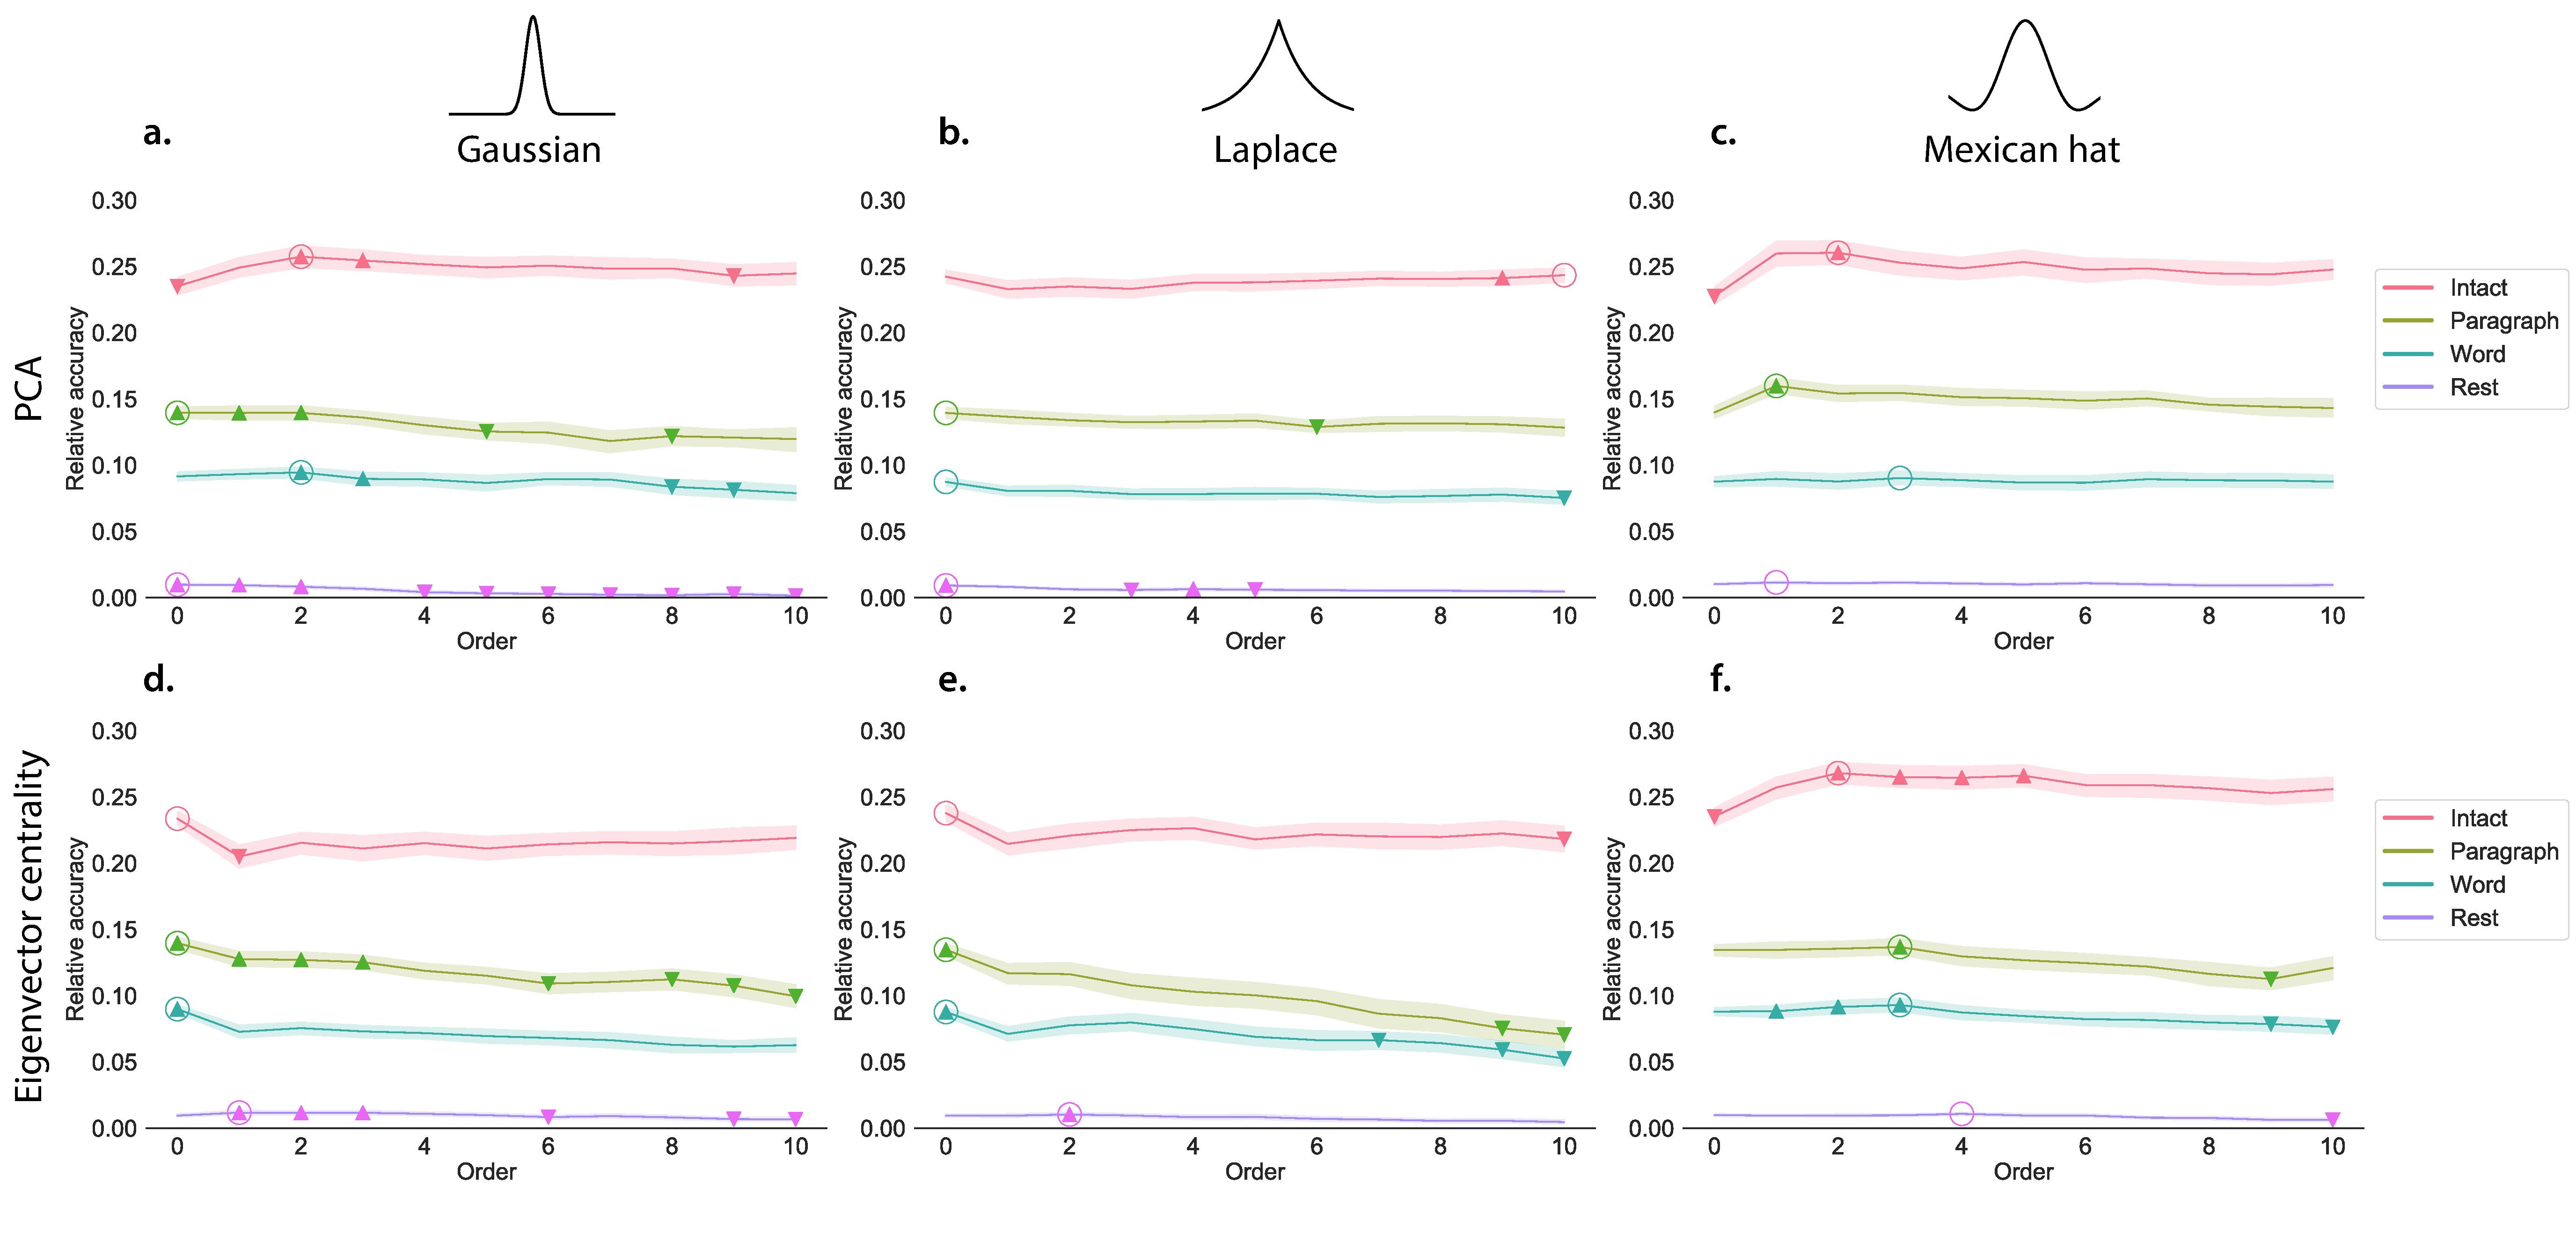
\includegraphics[width=0.95\textwidth]{figs/decode_levels_kernels}
\caption{\textbf{Across-participant decoding accuracy varies with
      correlation order and cognitive engagement across kernels.}
    \textbf{a.-c.~Decoding accuracy as a function of order: PCA.} \textit{Order} ($x$-axis) refers to the maximum order of dynamic
    correlations that were available to the classifiers (see
    \textit{Feature weighting and testing}).  The reported
    across-participant decoding accuracies for \textbf{a. Gaussian},
    \textbf{b. Laplace}, and \textbf{c. Mexican hat} kernels are averaged over all
   widths (see \textit{Identifying robust decoding
      results}).  The $y$-values are displayed relative to chance
    accuracy (intact: $\frac{1}{300}$; paragraph: $\frac{1}{272}$;
    word: $\frac{1}{300}$; rest: $\frac{1}{400}$).  The error ribbons
    denote 95\% confidence intervals across cross-validation folds
    (i.e., random assignments of participants to the training and test
    sets).  The colors denote the experimental condition.  Arrows
    denote sets of features that yielded reliably higher (upwards
    facing) or lower (downward facing) decoding accuracy than the mean
    of all other features (via a two-tailed test, thresholded at
    $p < 0.05$).  The circled values represent
    the maximum decoding accuracy within each experimental
    condition. Panels a.-c. used PCA to
    project each high-dimensional pattern of dynamic correlations onto
    a lower-dimensional space. \textbf{d.-f.~Decoding accuracy as a
      function of order: eigenvector centrality.} This panel is in the
    same format as Panel a.-c., but here eigenvector centrality has been
    used to project the high-dimensional patterns of dynamic
    correlations onto a lower-dimensional space.}
\label{fig:supp_kernels}
\end{figure}

\begin{figure}[p!]
\centering
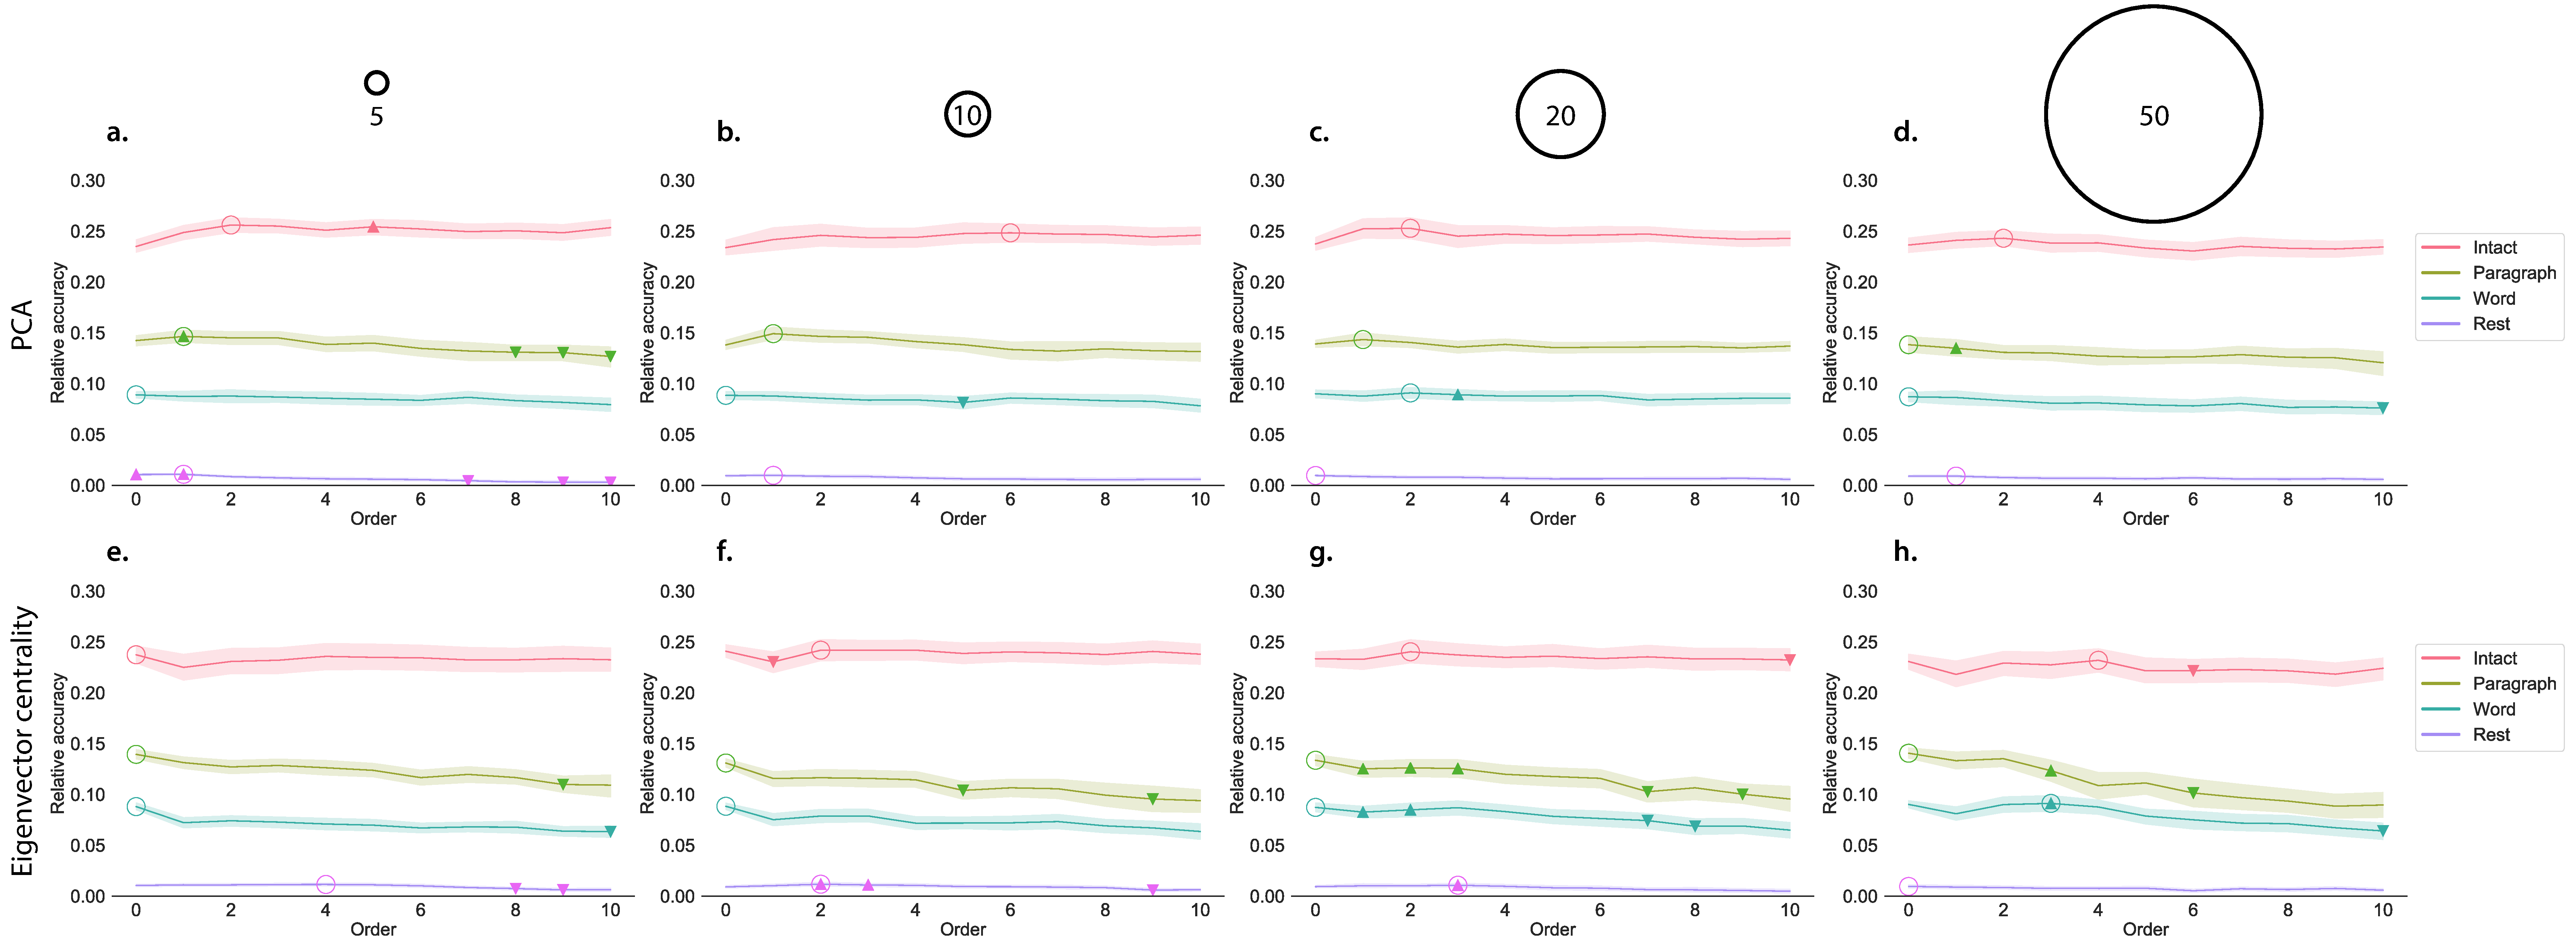
\includegraphics[width=0.95\textwidth]{figs/decode_levels_widths}
\caption{\textbf{Across-participant decoding accuracy varies with
      correlation order and cognitive engagement across widths.}
    \textbf{a.-d.~Decoding accuracy as a function of order: PCA.} \textit{Order} ($x$-axis) refers to the maximum order of dynamic
    correlations that were available to the classifiers (see
    \textit{Feature weighting and testing}).  The reported
    across-participant decoding accuracies for \textbf{a. 5},
    \textbf{b. 10}, \textbf{c. 20}, and \textbf{d. 50}  are averaged over all
    kernel shapes (see \textit{Identifying robust decoding
      results}).  The $y$-values are displayed relative to chance
    accuracy (intact: $\frac{1}{300}$; paragraph: $\frac{1}{272}$;
    word: $\frac{1}{300}$; rest: $\frac{1}{400}$).  The error ribbons
    denote 95\% confidence intervals across cross-validation folds
    (i.e., random assignments of participants to the training and test
    sets).  The colors denote the experimental condition.  Arrows
    denote sets of features that yielded reliably higher (upwards
    facing) or lower (downward facing) decoding accuracy than the mean
    of all other features (via a two-tailed test, thresholded at
    $p < 0.05$).  The circled values represent
    the maximum decoding accuracy within each experimental condition.  Panels a.-d. used PCA to
    project each high-dimensional pattern of dynamic correlations onto
    a lower-dimensional space.\textbf{e.-h.~Decoding accuracy as a
      function of order: eigenvector centrality.} This panel is in the
    same format as Panel a.-d., but here eigenvector centrality has been
    used to project the high-dimensional patterns of dynamic
    correlations onto a lower-dimensional space.}
\label{fig:supp_widths}
\end{figure}

\begin{figure}[p!]
\centering
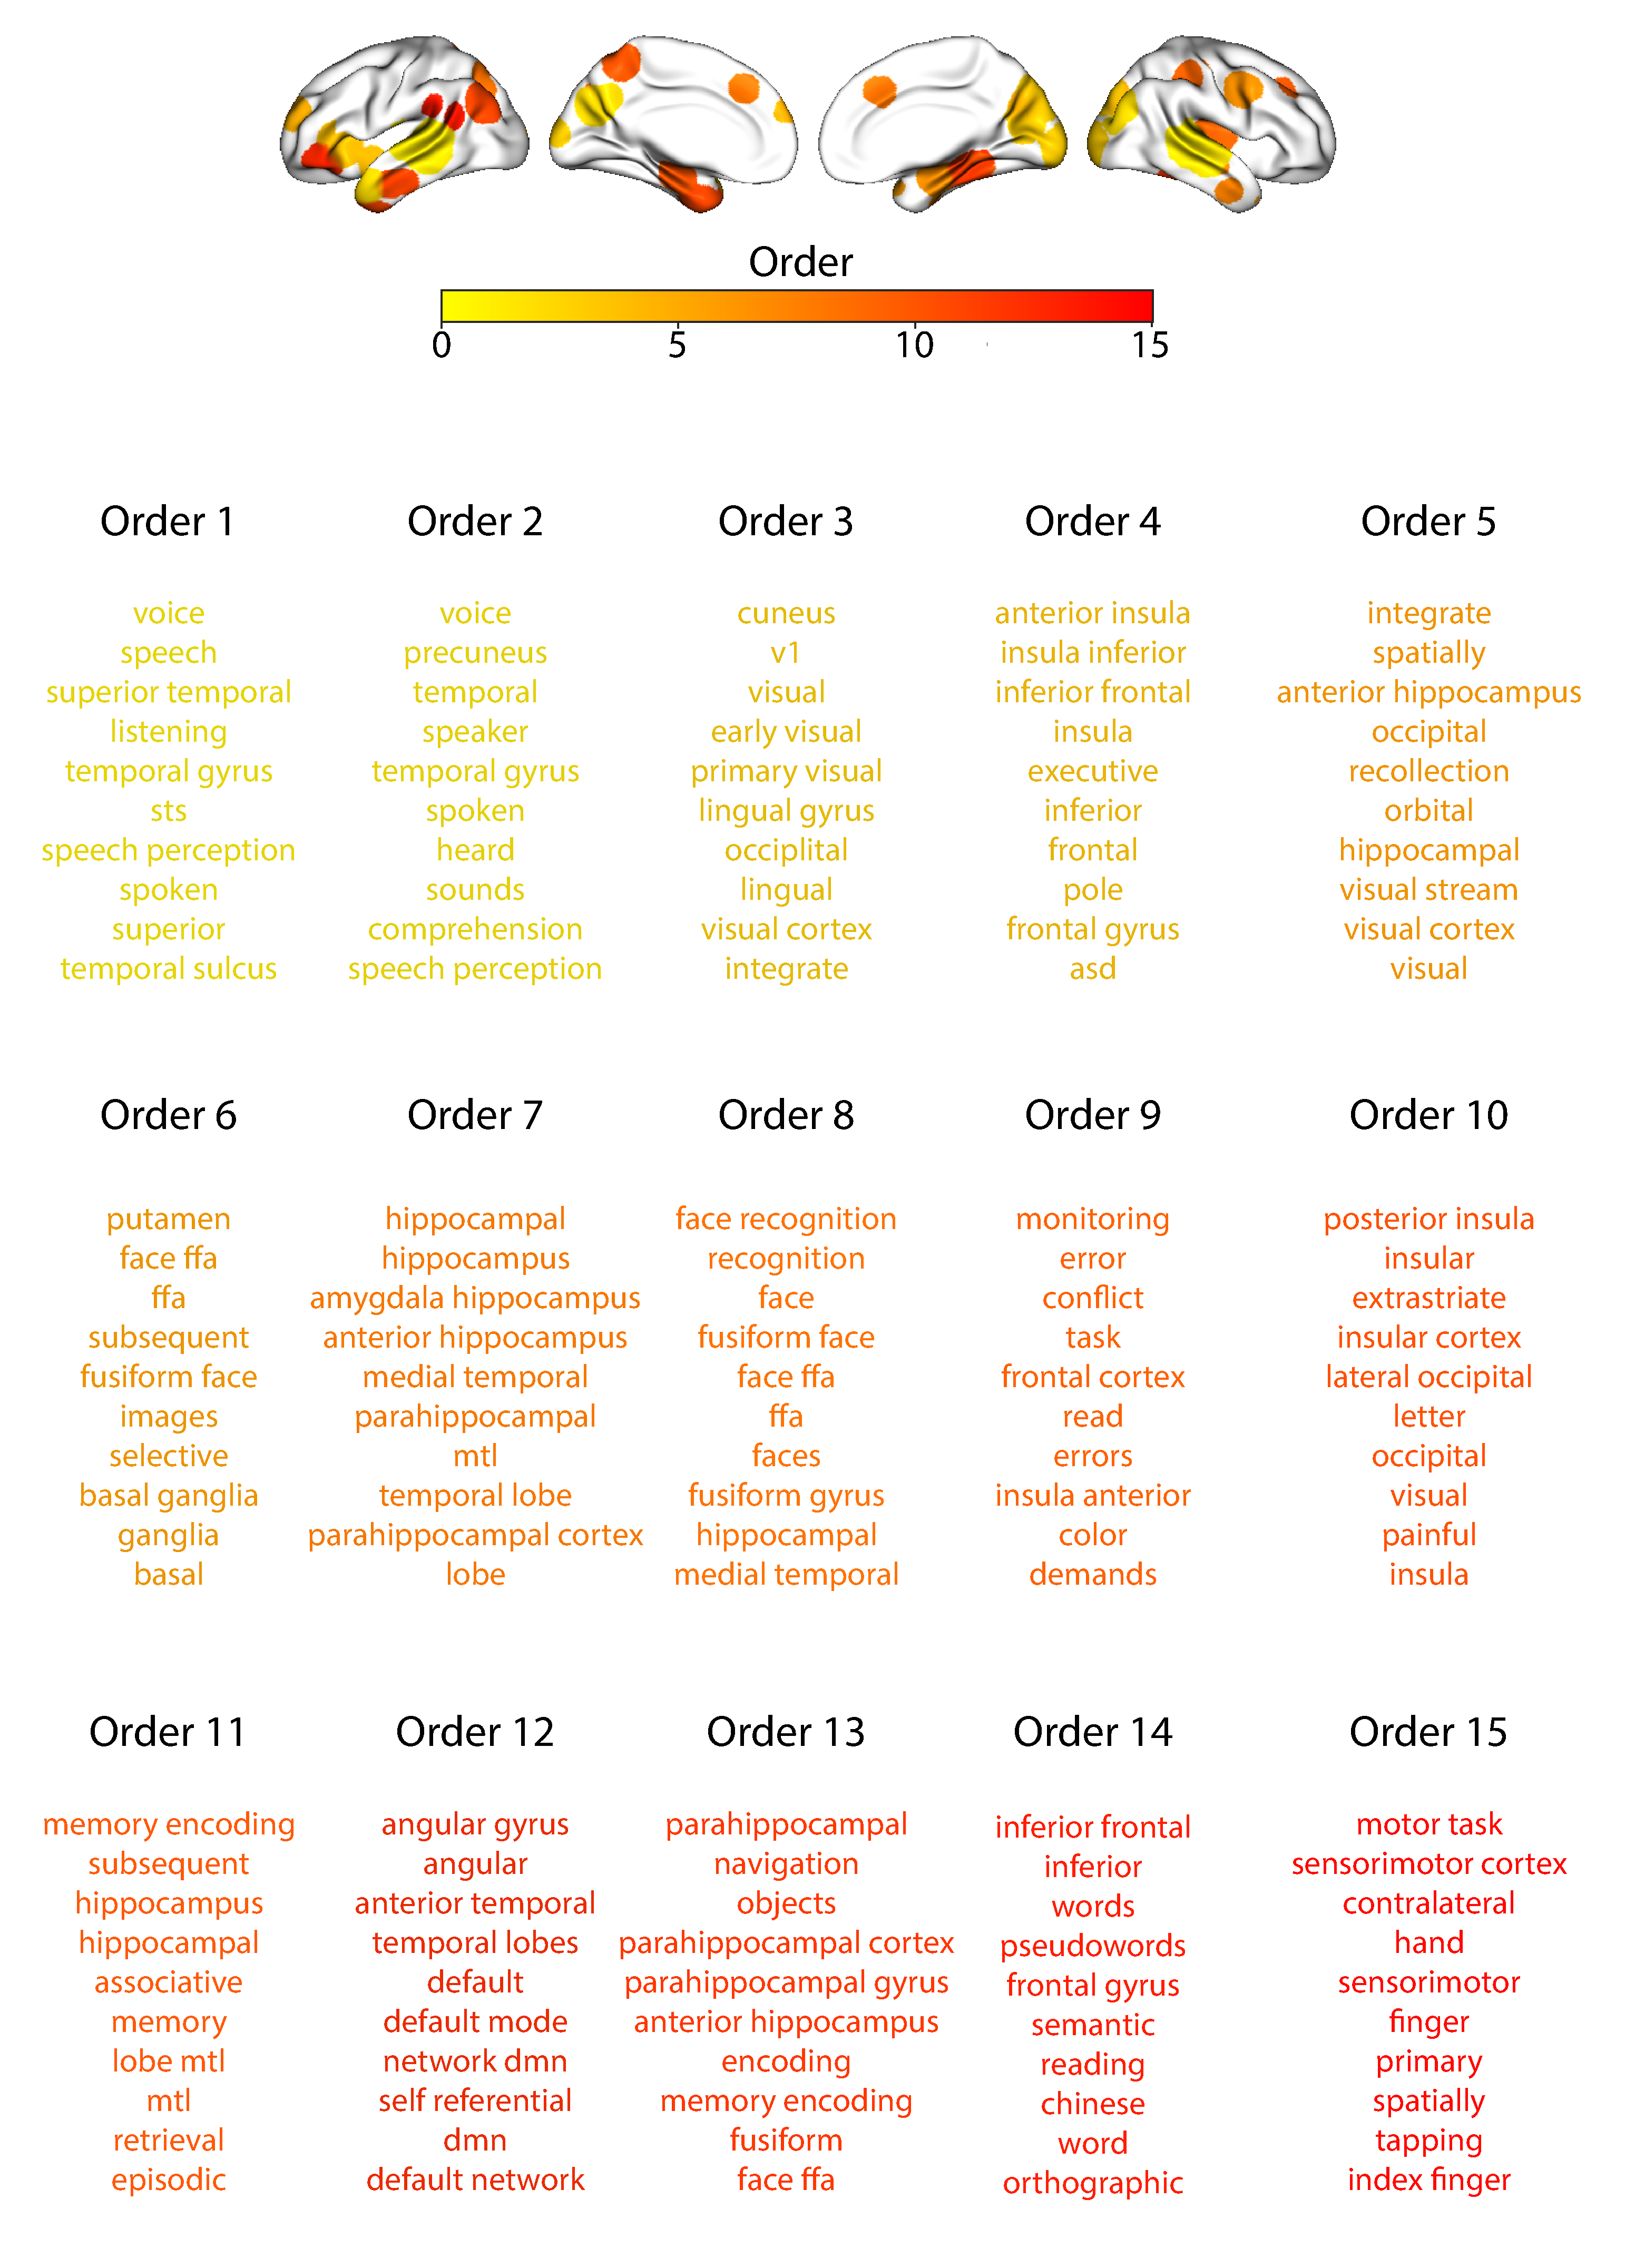
\includegraphics[width=0.75\textwidth]{figs/supp_15_intact}
\caption{\textbf{Top terms associated with the endpoints of the
    strongest correlations for the \textit{intact} experimental
    condition.}  Each color corresponds to one order of inter-subject
functional correlations. The inflated brain plots display the
locations of the endpoints of the 10 strongest (absolute value)
correlations at each order, projected onto the cortical
surface~\citep{CombEtal19}.  The lists of terms display
the top 10 Neurosynth terms~\citep{RubiEtal17} decoded from the
corresponding brain maps for each order.  (Also see Fig.~\neurosynth,
top row, in the main text.)}
\label{fig:intact}
\end{figure}

\begin{figure}[p!]
\centering
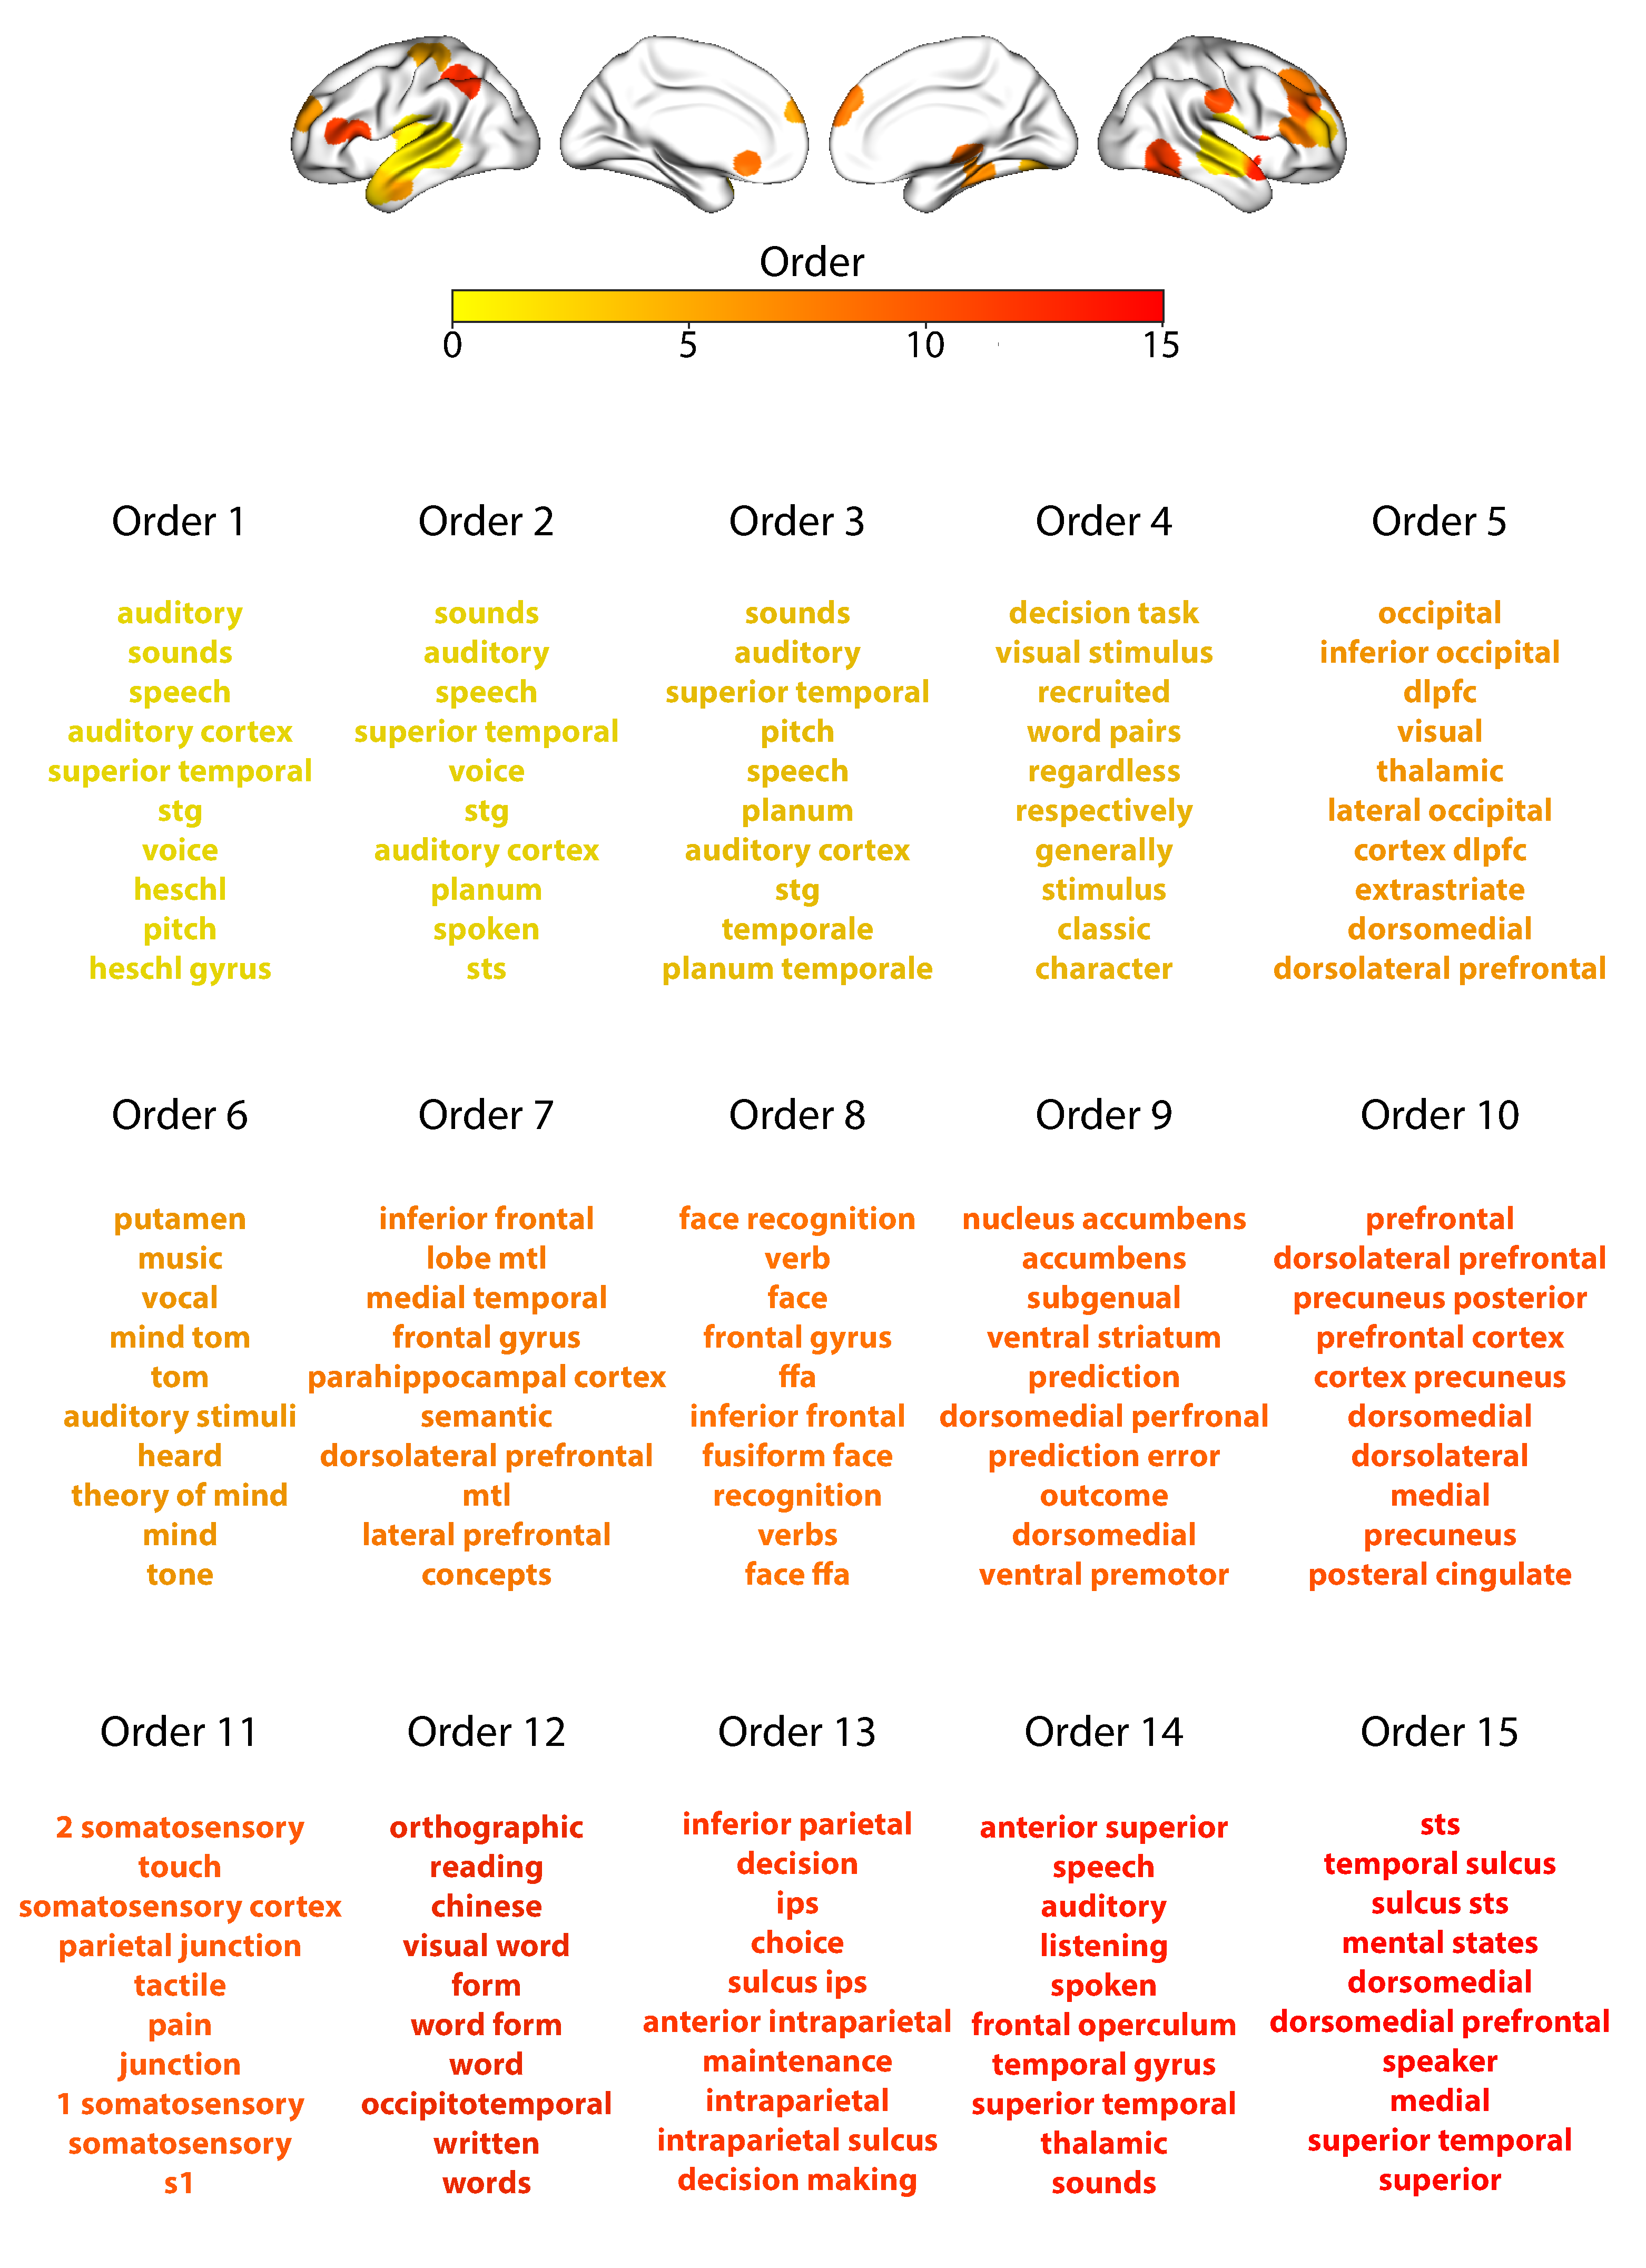
\includegraphics[width=0.75\textwidth]{figs/supp_15_paragraph}
\caption{\textbf{Top terms associated with the endpoints of the
    strongest correlations for the \textit{paragraph} experimental
    condition.}  This figure is in the same format as
  Figure~\ref{fig:intact}, but displays results for the
  paragraph-scrambled story listening condition.  (Also see Fig.~\neurosynth,
second row, in the main text.)}
\label{fig:paragraph}
\end{figure}

\begin{figure}[p!]
\centering
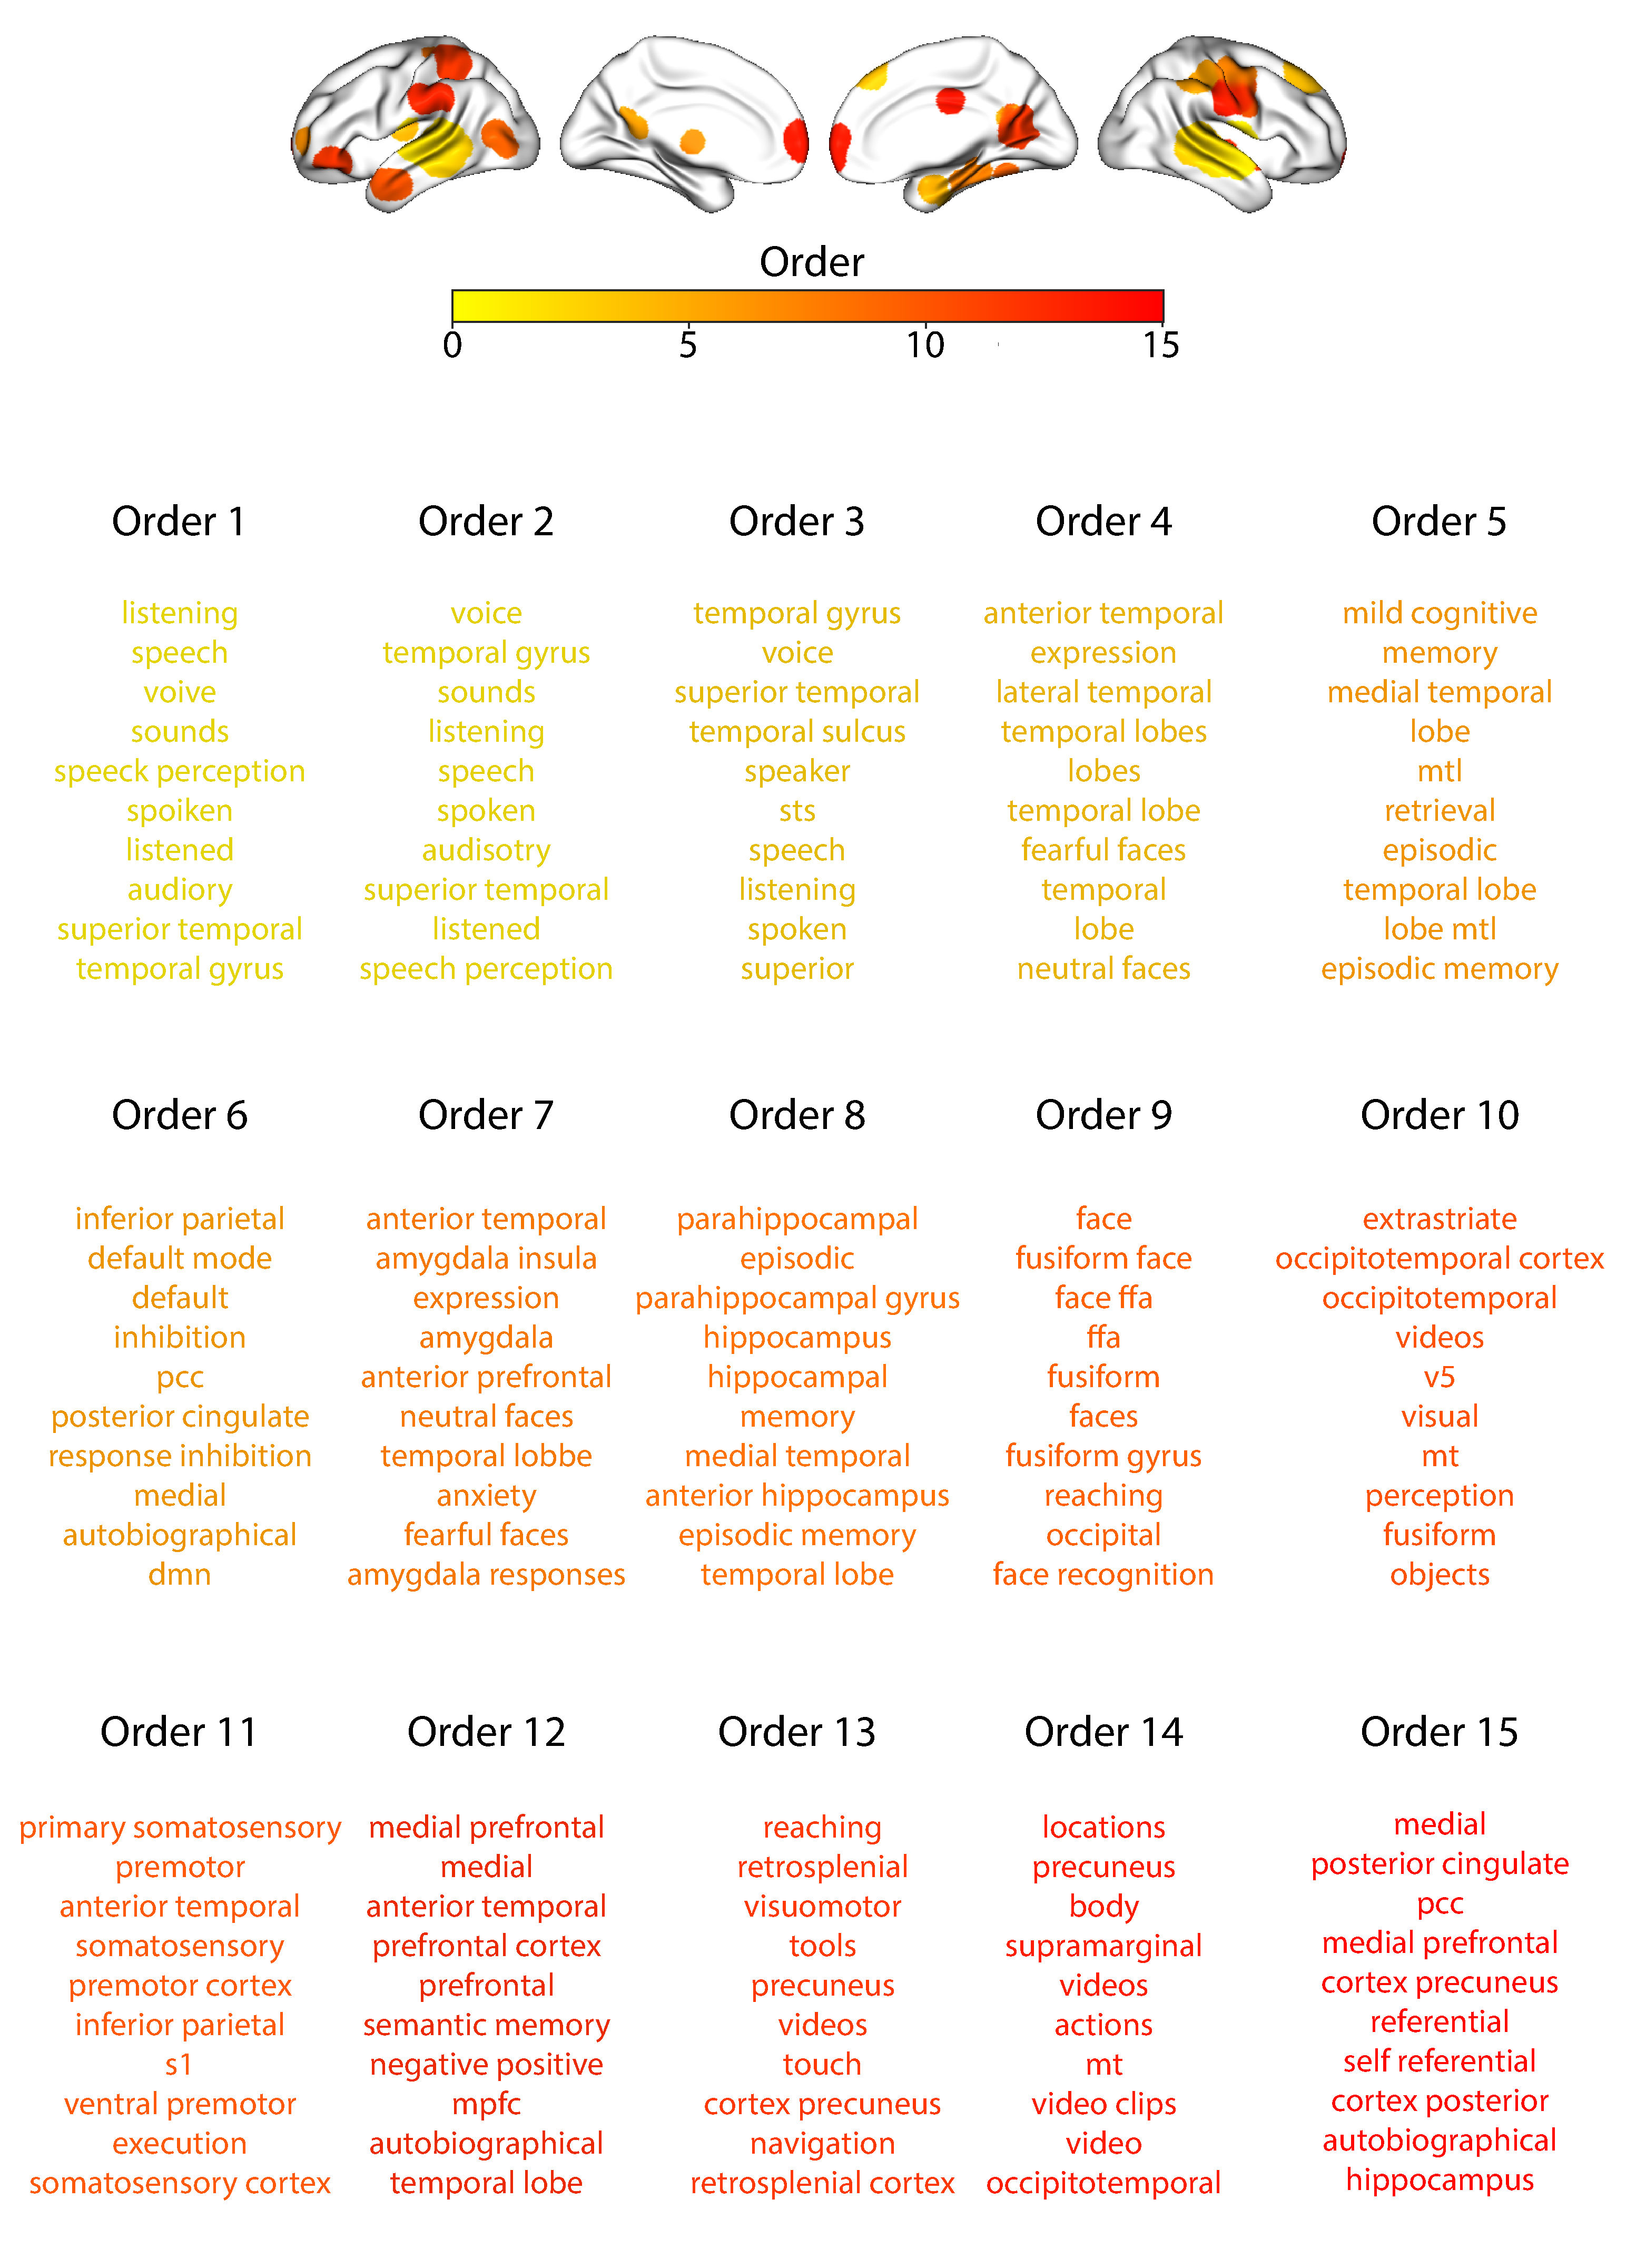
\includegraphics[width=0.75\textwidth]{figs/supp_15_word}
\caption{\textbf{Top terms associated with the endpoints of the
    strongest correlations for the \textit{word} experimental
    condition.}  This figure is in the same format as
  Figure~\ref{fig:intact}, but displays results for the
  word-scrambled story listening condition.  (Also see Fig.~\neurosynth,
third row, in the main text.)}
\label{fig:word}
\end{figure}

\begin{figure}[p!]
\centering
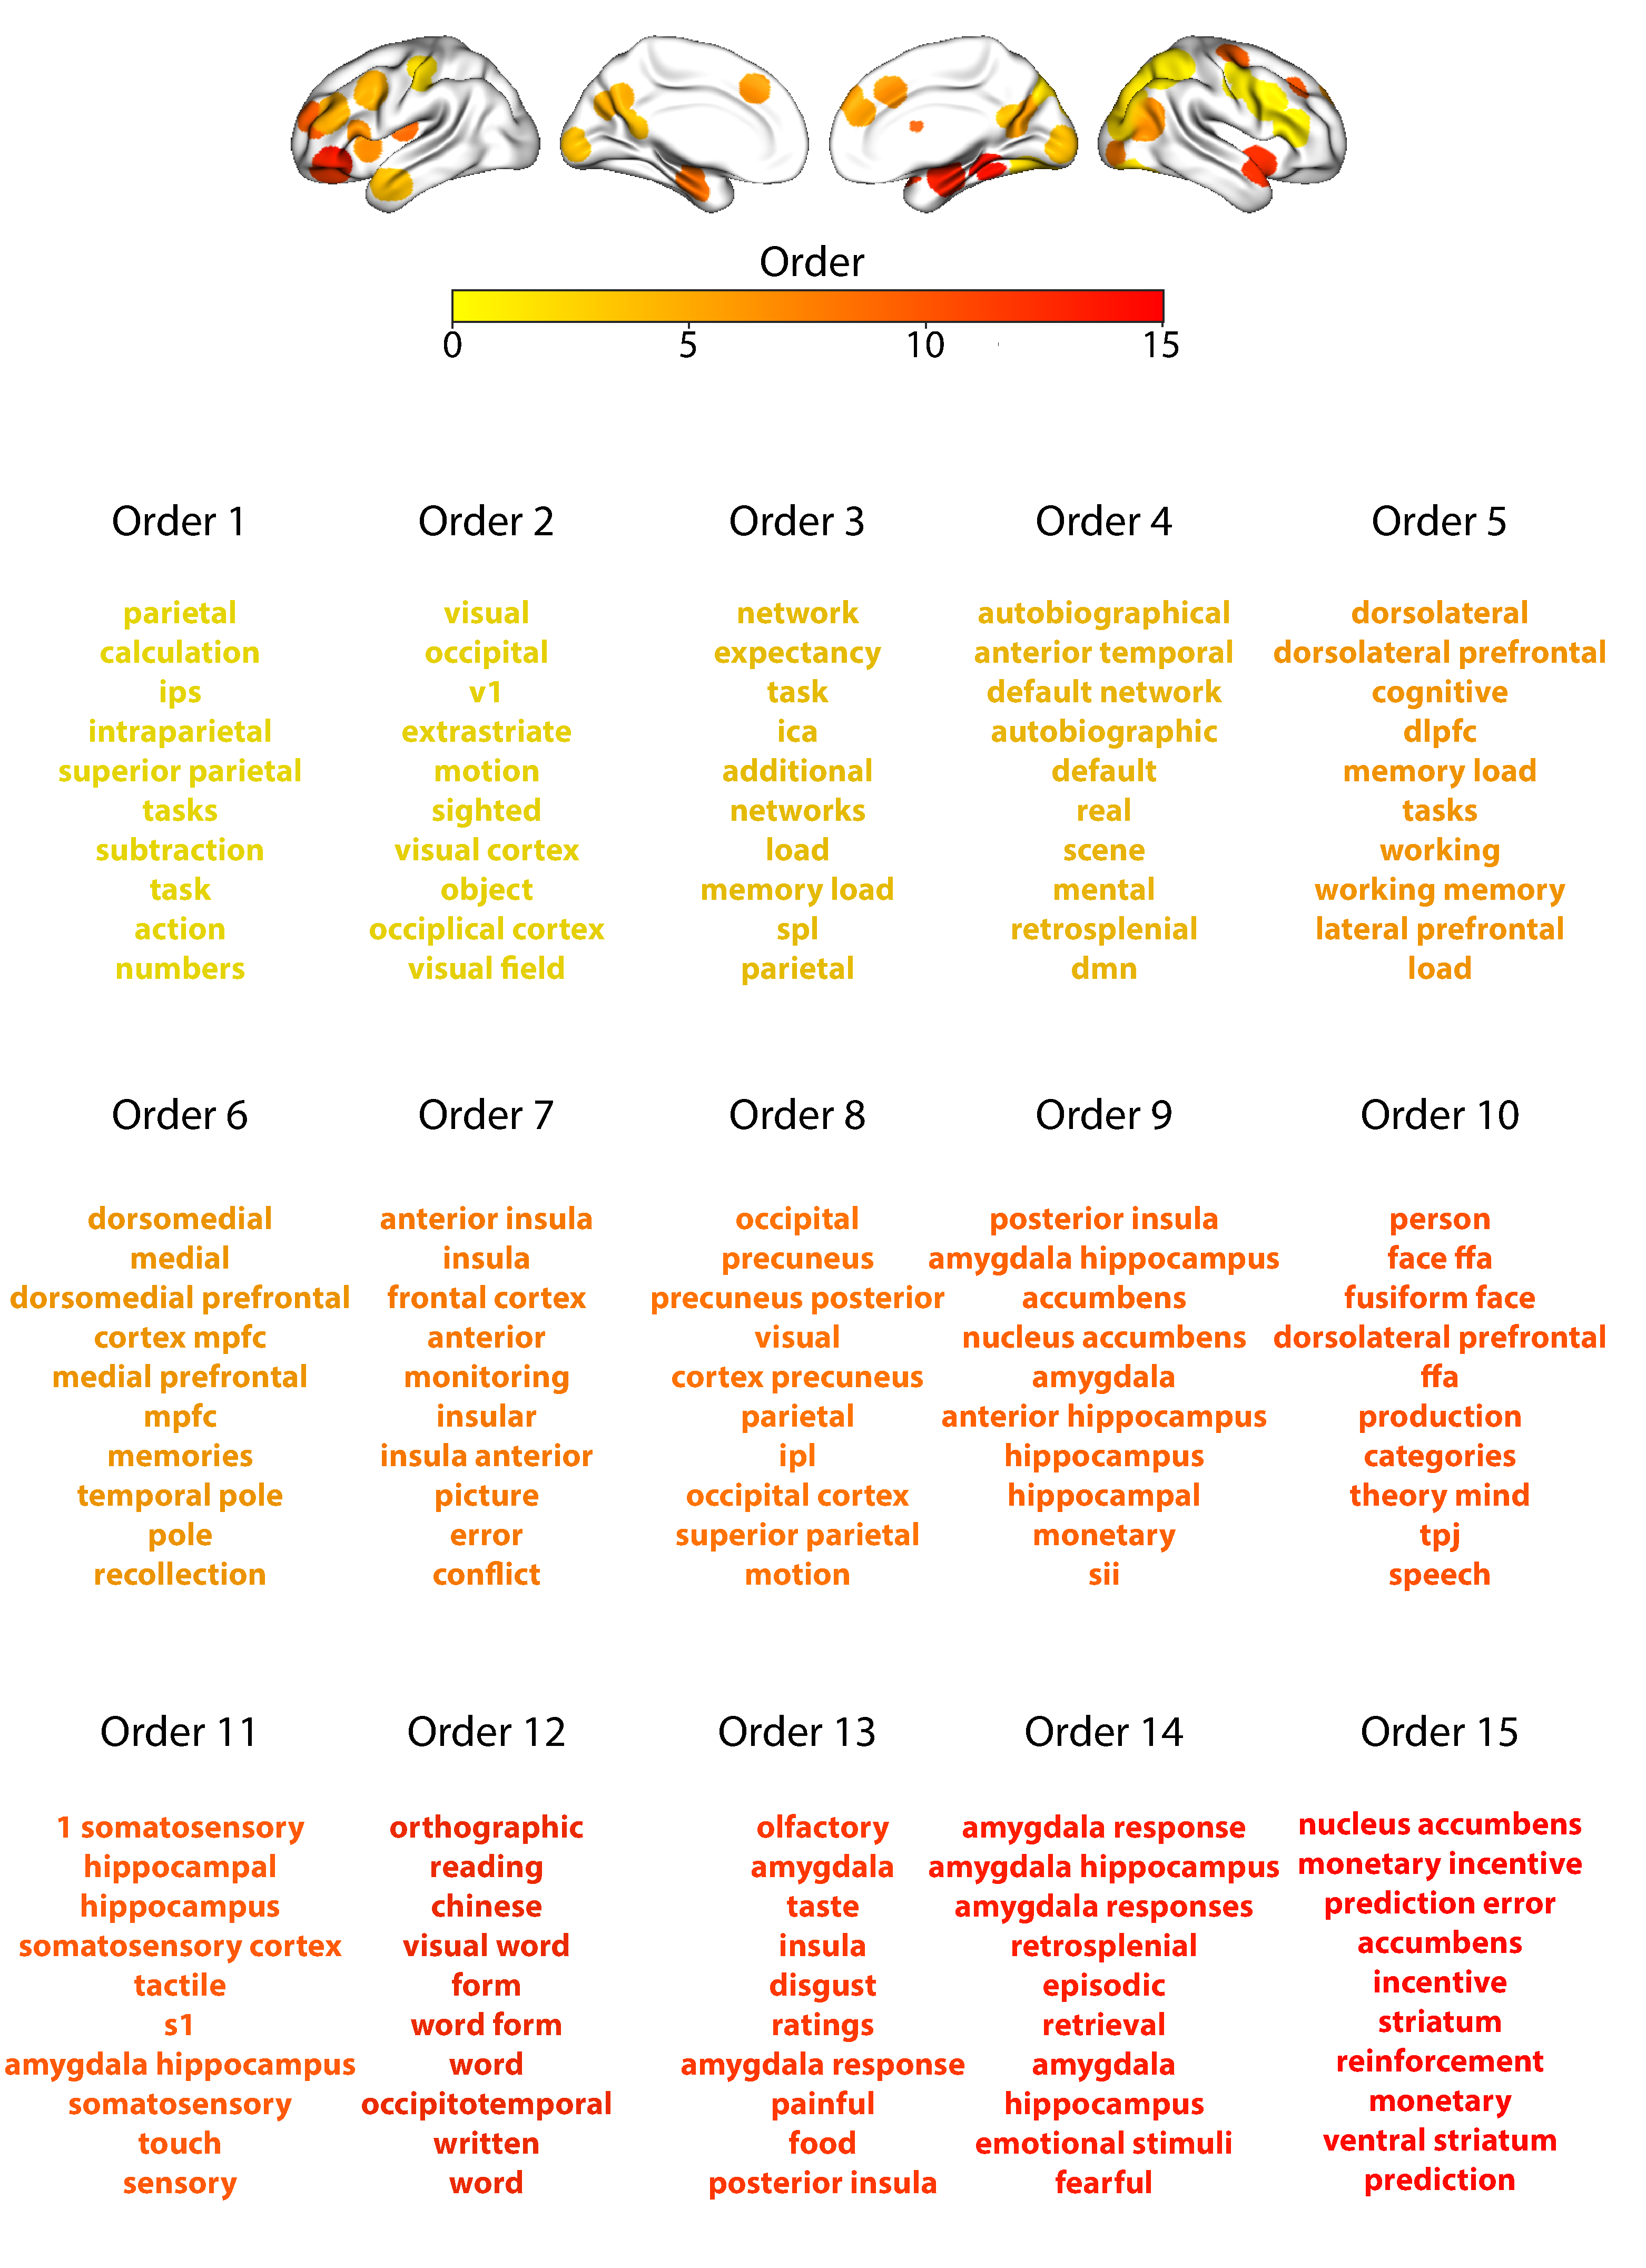
\includegraphics[width=0.75\textwidth]{figs/supp_15_rest}
\caption{\textbf{Top terms associated with the endpoints of the
    strongest correlations for the \textit{rest} experimental
    condition.}  This figure is in the same format as
  Figure~\ref{fig:intact}, but displays results for the
  resting state condition.  (Also see Fig.~\neurosynth,
bottom row, in the main text.)}
\label{fig:rest}
\end{figure}

\begin{figure}[p!]
\centering
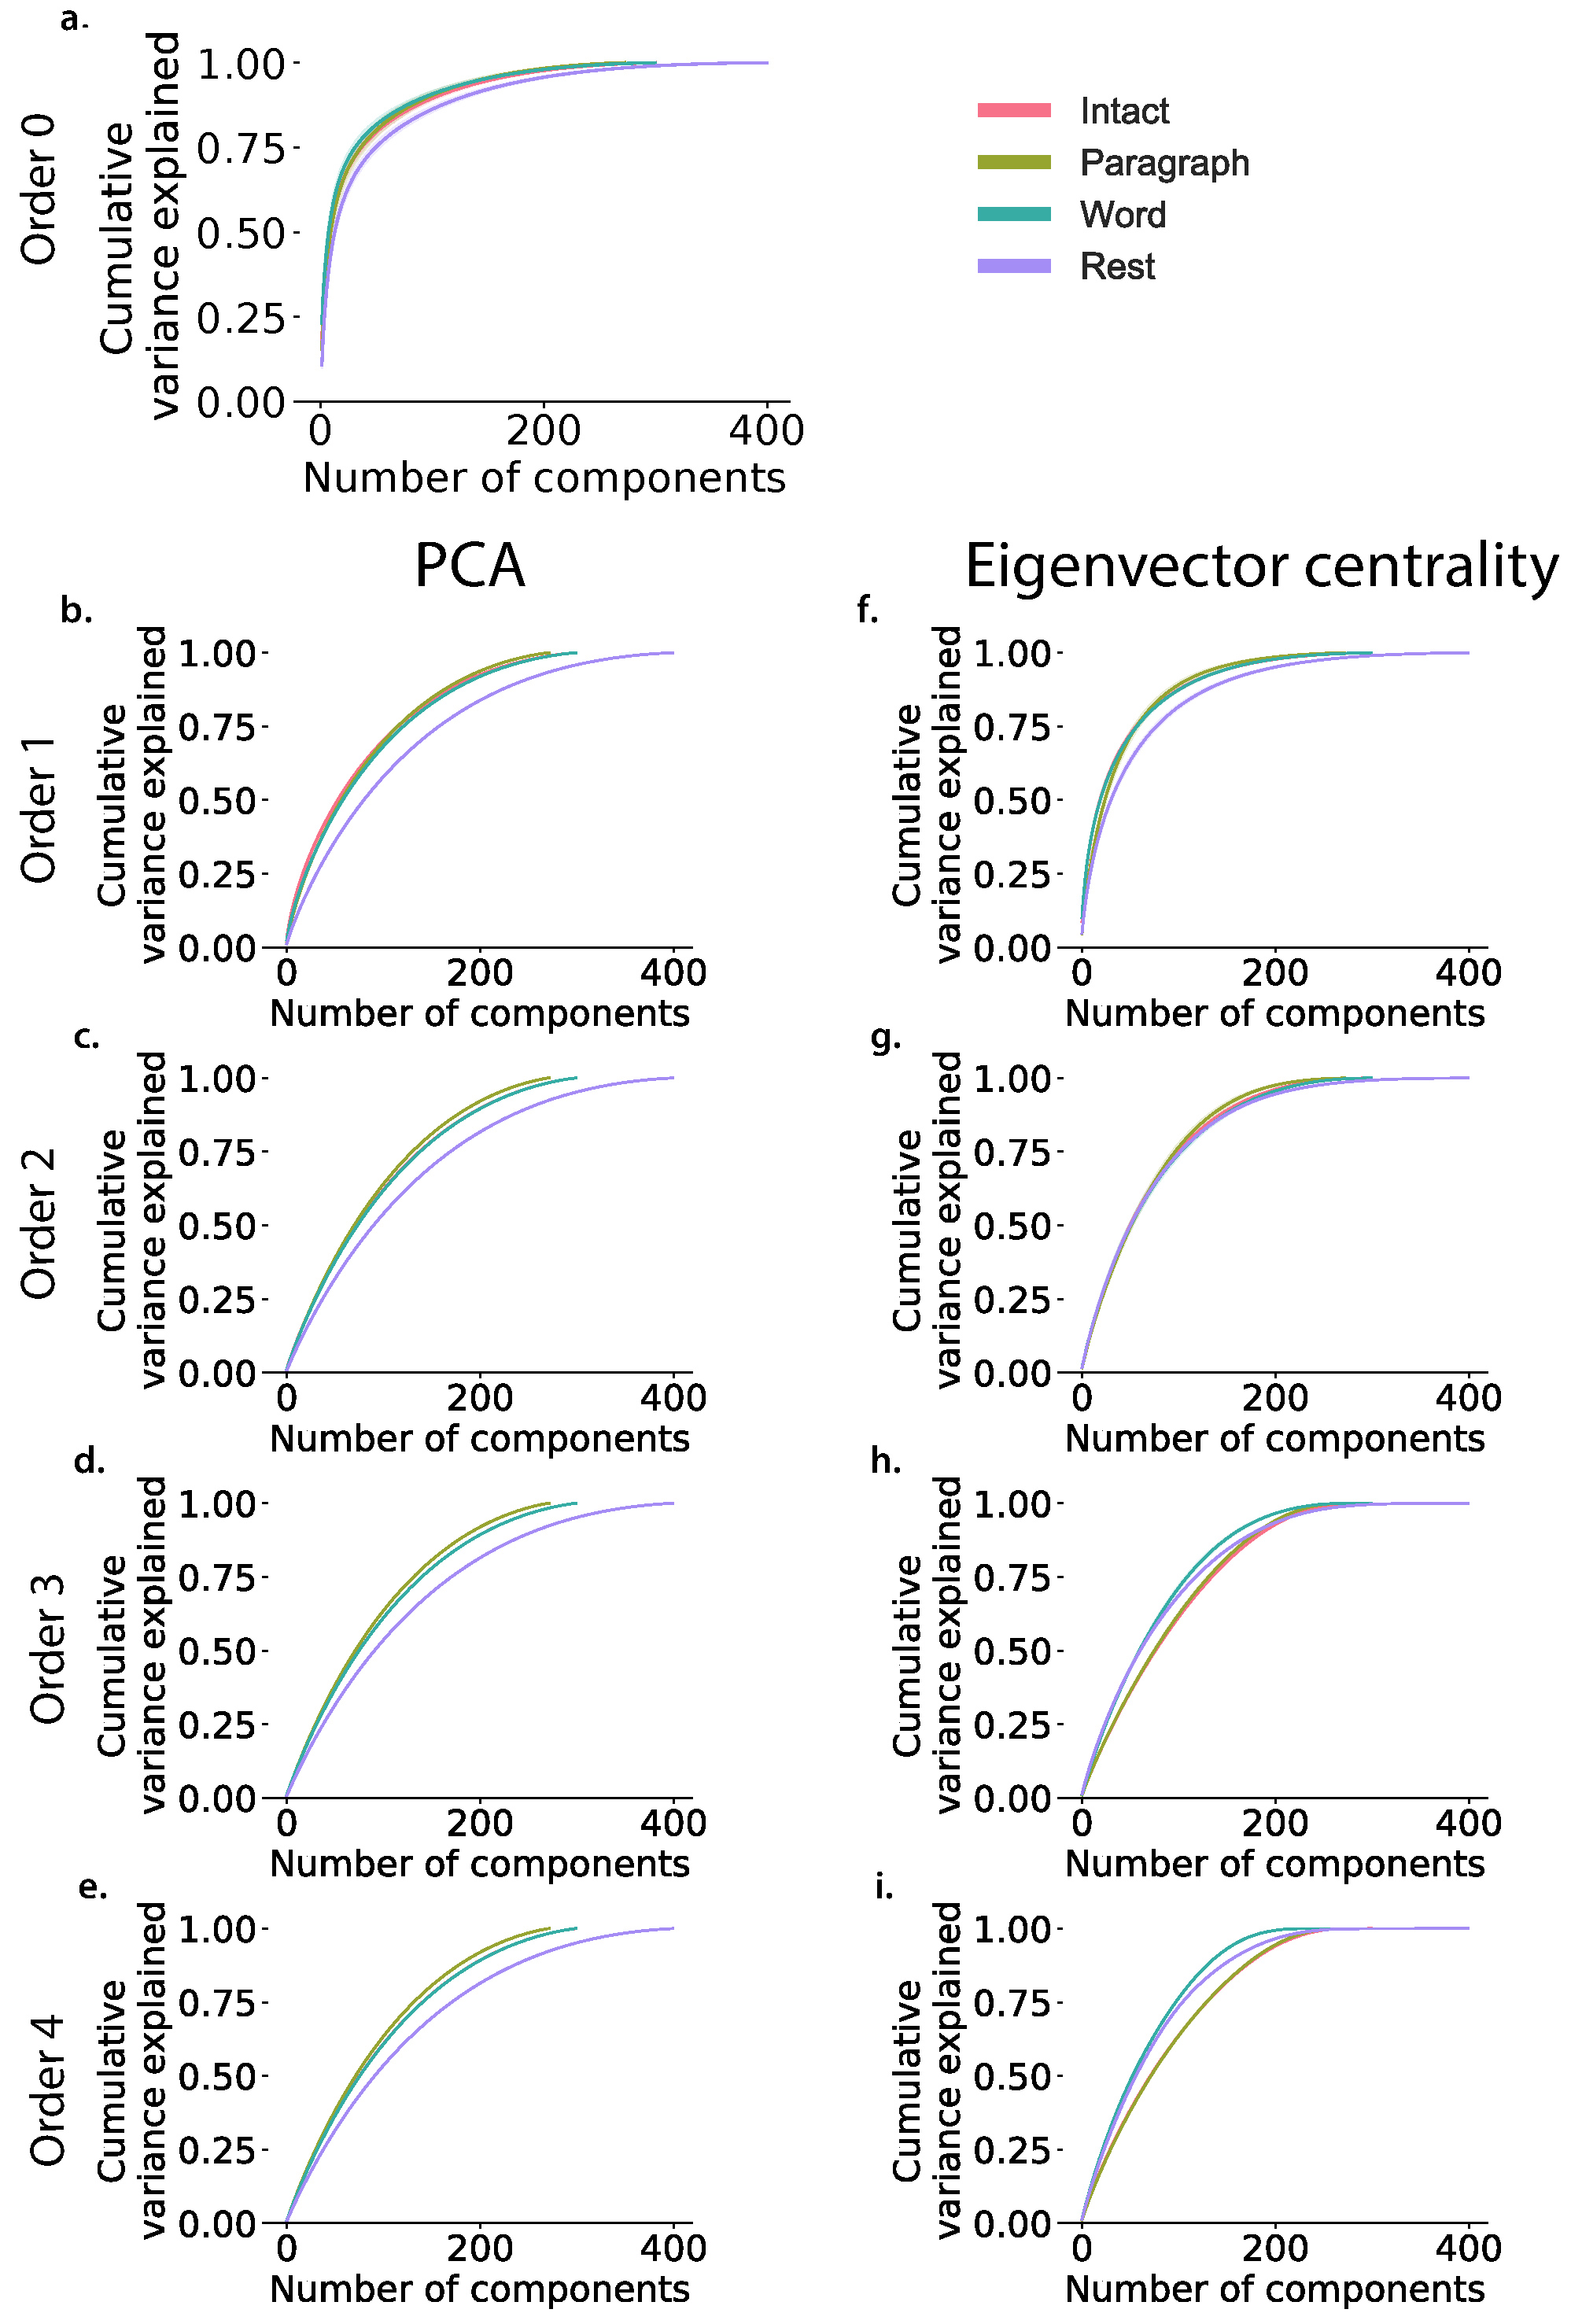
\includegraphics[width=0.75\textwidth]{figs/pca}
\caption{\textbf{Cumulative percent variance explained as a function
    of the number of principle components for correlation orders and reduction types.}  \textit{Order} refers to the order of the dynamic
    correlations calculated. Principle components analysis was
    performed, and reduced independently for each subject.  Maximum number of components varies with
    the total time for each condition (intact: 300; paragraph:272;
    word: 300; rest: 400). \textbf{a.~Cumlative percent
    variance as a function of number of components for Order 0.} PCA
  was performed on the raw acitivity patterns (Order 0). \textbf{b.-e.~Cumlative percent
    variance as a function of number of components for Orders 1.-4.:
    PCA} Dynamic correlation were calculated for orders 1-4 using PCA to
    project each high-dimensional pattern of dynamic correlations onto
    a lower-dimensional space.   \textbf{f.-i.~Cumlative percent
    variance as a function of number of components for Orders 1.-4.: eigenvector centrality.} These panels arer in the
    same format as Panel b.-e., but here eigenvector centrality has been
    used to project the high-dimensional patterns of dynamic
    correlations onto a lower-dimensional space. }
\label{fig:pca}
\end{figure}


%\section*{Participant-level figures referenced in the main text}

% Supporting information


\newpage
\renewcommand{\refname}{Supplemental references}
\bibliography{memlab}


\end{document}